\documentclass[10pt,aspectratio=169]{beamer}

% All the boilerplate is in raslides.sty
% Note that this also pulls in a custom vogtwidebar.sty
\usepackage{raslides}

\author{Ji\v{r}\'i Lebl}

\institute[OSU]{%
Departemento pri Matematiko de Oklahoma {\^S}tata Universitato}

\title{BA: 7.1}

\date{}

\begin{document}

\begin{frame}
\titlepage
\end{frame}

\begin{frame}
We wish to generalize convergence, continuity, etc.

\pause

\begin{definition}
Let $X$ be a set, and let
$d \colon X \times X \to \R$
be such that for all $x,y,z \in X$
\begin{enumerate}[(i)]
%
\item \label{metric:pos}
\pause
\makebox[2.0in][l]{$d(x,y) \geq 0$.}
(\emph{nonnegativity})
%
\item \label{metric:zero}
\pause
\makebox[2.0in][l]{$d(x,y) = 0$ \wiffif $x = y$.}
(\emph{identity of indiscernibles})
%
\item \label{metric:com}
\pause
\makebox[2.0in][l]{$d(x,y) = d(y,x)$.} 
(\emph{symmetry})
%
\item \label{metric:triang}
\pause
\makebox[2.0in][l]{$d(x,z) \leq d(x,y)+ d(y,z)$.}
(\emph{triangle inequality})
\end{enumerate}

\pause
\medskip

$(X,d)$ is called a \emph{metric space}.

\pause
\medskip
  
$d$ is called the \emph{metric} or the \emph{distance function}.

\pause
\medskip

Sometimes write just $X$ instead of $(X,d)$
if the metric is clear from context.
\end{definition}

\pause
Think of $d$ as a distance between points.

\pause
\medskip

\eqref{metric:pos}--\eqref{metric:com} have obvious geometric
interpretation.

\end{frame}

\begin{frame}

The interpretation of triangle inequality:

\medskip

\begin{center}
\scalebox{0.8}{
\subimport*{../figures/}{ms-triang.pdf_t}
}
\end{center}

\pause
\medskip

\textbf{Warning:}
It is convenient to draw figures and diagrams in the plane,
but that is just one particular metric space!

\end{frame}

\begin{frame}

\textbf{Example:}
$\R$ is a metric space with the metric
\quad $d(x,y) \coloneqq \abs{x-y}$.

\pause
\eqref{metric:pos}--\eqref{metric:com} are easy to verify.
\pause
\quad
For triangle inequality, \eqref{metric:triang}:
\begin{equation*}
d(x,z)
\pause
= \abs{x-z}
\pause
= 
\abs{x-y+y-z}
\pause
\leq
\abs{x-y}+\abs{y-z}
\pause
=
d(x,y)+ d(y,z) .
\end{equation*}
\pause
$d$ is the \emph{standard metric on $\R$}.
\pause
\quad (It's the default one if none mentioned.)

\pause
\medskip

\textbf{Example:}
We can also have a different metric on $\R$.
\pause
E.g.,
~
$
d(x,y)
\coloneqq
\dfrac{\abs{x-y}}{\abs{x-y}+1}$.

\pause
\eqref{metric:pos}--\eqref{metric:com} are again easy.
\pause
\quad
For triangle

inequality, \eqref{metric:triang}, note
$d(x,y) = \varphi(\abs{x-y})$,

where $\varphi(t) = \frac{t}{t+1}$ and
$\varphi$ is increasing.

\vspace*{-0.5in}
\hspace*{2.7in}
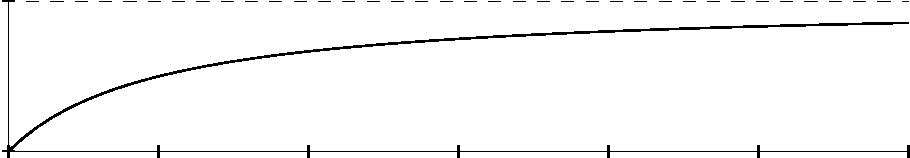
\includegraphics[height=0.5in]{../figures/tovertp1graph}

\vspace*{-0.05in}

\pause
\medskip

$
d(x,z)
\pause
=
\varphi(\abs{x-z})
\pause
= 
\varphi(\abs{x-y+y-z})
\pause
\leq
\varphi(\abs{x-y}+\abs{y-z})
$

\pause
\medskip

\qquad
$
=
\dfrac{\abs{x-y}+\abs{y-z}}{\abs{x-y}+\abs{y-z}+1}
\pause
=
\dfrac{\abs{x-y}}{\abs{x-y}+\abs{y-z}+1} +
\dfrac{\abs{y-z}}{\abs{x-y}+\abs{y-z}+1}
$

\pause
\medskip

\qquad
$
\leq
\dfrac{\abs{x-y}}{\abs{x-y}+1} +
\dfrac{\abs{y-z}}{\abs{y-z}+1}
\pause
=
d(x,y)+ d(y,z)$.

\pause
\medskip

With this metric, $d(x,y) < 1$ for all $x,y \in \R$.

\end{frame}

\begin{frame}
$\R^n = \R \times \R \times \cdots \times \R$
is the
$n$-dimensional \emph{euclidean space}.

\pause
Notation for points: ~~~ $x =(x_1,x_2,\ldots,x_n) \in \R^n$.
\pause
\qquad (We don't write $\vec{x}$ nor $\mathbf{x}$)

\pause
We also write $0 \in \R^n$ to mean $(0,0,\ldots,0)$.

\pause

\begin{lemma}[Cauchy--Schwarz inequality]
If $x =(x_1,x_2,\ldots,x_n) \in \R^n$, $y =(y_1,y_2,\ldots,y_n) \in
\R^n$, then
\begin{equation*}
{\biggl( \sum_{k=1}^n x_k y_k \biggr)}^2
\leq
\biggl(\sum_{k=1}^n x_k^2 \biggr)
\biggl(\sum_{k=1}^n y_k^2 \biggr) .
\end{equation*}
\end{lemma}

\pause
\textbf{Proof:}
A square of a real number is nonnegative.
\pause
Hence,

\medskip

$
0
\leq 
\sum_{k=1}^n \sum_{\ell=1}^n {(x_k y_\ell - x_\ell y_k)}^2
\pause
=
\sum_{k=1}^n \sum_{\ell=1}^n
\bigl( x_k^2 y_\ell^2 + x_\ell^2 y_k^2 - 2 x_k x_\ell y_k y_\ell \bigr)
$

\pause
\medskip

\quad
$=
\biggl( \sum_{k=1}^n x_k^2 \biggr)
\biggl( \sum_{\ell=1}^n y_\ell^2 \biggr)
+
\biggl( \sum_{k=1}^n y_k^2 \biggr)
\biggl( \sum_{\ell=1}^n x_\ell^2 \biggr)
-
2
\biggl( \sum_{k=1}^n x_k y_k \biggr)
\biggl( \sum_{\ell=1}^n x_\ell y_\ell \biggr)$.

\pause
\medskip

\thus \quad 
$0 \leq 
\biggl( \sum_{k=1}^n x_k^2 \biggr)
\biggl( \sum_{k=1}^n y_k^2 \biggr)
-
{\biggl( \sum_{k=1}^n x_k y_k \biggr)}^2$.
\qed

\end{frame}

\begin{frame}

\textbf{Example:}
We define the
standard metric for $\R^n$:
\begin{equation*}
d(x,y) \coloneqq
\sqrt{
{(x_1-y_1)}^2 + 
{(x_2-y_2)}^2 + 
\cdots +
{(x_n-y_n)}^2
} =
\sqrt{
\sum_{k=1}^n
{(x_k-y_k)}^2 
} .
\end{equation*}
\pause
\textbf{Note:} If $n=1$ agrees with above.

\pause
\medskip

The only tricky bit (again) is to check triangle inequality.

\pause
\medskip

$
{\bigl(d(x,z)\bigr)}^2
\pause
=
\sum_{k=1}^n
{(x_k-z_k)}^2 
\pause
=
\sum_{k=1}^n
{(x_k-y_k+y_k-z_k)}^2 
$

\pause
\medskip

\quad
$
=
\sum_{k=1}^n
\Bigl(
{(x_k-y_k)}^2+{(y_k-z_k)}^2 + 2(x_k-y_k)(y_k-z_k)
\Bigr)
$

\pause
\medskip

\quad
$
=
\sum_{k=1}^n
{(x_k-y_k)}^2
+
\sum_{k=1}^n
{(y_k-z_k)}^2 
+
2
\sum_{k=1}^n
(x_k-y_k)(y_k-z_k)
$

\pause
\medskip

\quad
$
\leq
\sum_{k=1}^n
{(x_k-y_k)}^2
+
\sum_{k=1}^n
{(y_k-z_k)}^2 
+
2
\sqrt{
\sum_{k=1}^n
{(x_k-y_k)}^2
\sum_{k=1}^n
{(y_k-z_k)}^2
}
$

\pause
\medskip

\quad
$
=
{\left(
\sqrt{
\sum_{k=1}^n
{(x_k-y_k)}^2
}
+
\sqrt{
\sum_{k=1}^n
{(y_k-z_k)}^2 
}
\right)}^2
\pause
=
{\bigl( d(x,y) + d(y,z) \bigr)}^2$.

\pause
\medskip

The triangle inequality follows as $\sqrt{\cdot}$ is an increasing function.

\end{frame}

\begin{frame}

\textbf{Example:}
Complex numbers $\C$ is the set of numbers $z = x+iy$, where $x,y \in \R$.

\pause
\medskip

Imposing $i^2 = -1$, makes $\C$ into a field.

\pause
\medskip

To make $\C$ into a metric space, identify $\C$ with $\R^2$ by
\[
x+iy \in \C \quad \leftrightarrow \quad (x,y) \in \R^2 ,
\]
and use the standard metric.

\pause
\medskip

Define the \emph{complex modulus} $\sabs{x+iy} \coloneqq \sqrt{x^2+y^2}$.

\pause
\medskip

If $z_1 = x_1 + iy_1$ and $z_2 = x_2 + iy_2$, then
\[
d(z_1,z_2) = \sqrt{{(x_1-x_2)}^2+ {(y_1-y_2)}^2} = \sabs{z_1-z_2}.
\]
%Furthermore, when working with complex numbers
%it is often convenient to write the metric in terms of
%the so-called
%\emph{complex conjugate}: The conjugate of $z=x+iy$
%is $\bar{z} \coloneqq x-iy$.  Then 
%${\sabs{z}}^2 = x^2 +y^2 = z\bar{z}$, and so ${\sabs{z_1-z_2}}^2 =
%(z_1-z_2)\overline{(z_1-z_2)}$.
\end{frame}

\begin{frame}

\textbf{Example:}
For any set $X$, define the \emph{discrete metric}:
\begin{equation*}
d(x,y) \coloneqq
\begin{cases}
1 & \text{if } x \not= y, \\
0 & \text{if } x = y.
\end{cases}
\end{equation*}
\pause
Easy to check the properties.

\pause
\medskip

E.g., if $X = \{ a,b,c,d,e \}$, then

\begin{center}
\scalebox{0.8}{
\subimport*{../figures/}{msdiscmetric.pdf_t}
}
\end{center}

\pause
A very useful 
``smell test'' for statements about metric spaces.
\end{frame}

\begin{frame}

\textbf{Example:}
Let $C\bigl([a,b],\R\bigr)$ be the set of
continuous functions $f \colon [a,b] \to \R$.
\pause
Define the (standard) metric as
\qquad $
d(f,g) \coloneqq \sup\limits_{x \in [a,b]} \abs{f(x)-g(x)}$.

\pause
\medskip

$d(f,g)$ is finite as $\abs{f(x)-g(x)}$ is a continuous function on a closed bounded interval
$[a,b]$ and so bounded.

\pause
\medskip

(i) \quad Clearly $d(f,g) \geq 0$. 

\pause
\medskip

(ii) \quad $f = g$
\pause
\wthus $\forall x$, $\abs{f(x)-g(x)} = 0$
\pause
\wthus $d(f,g) = 0$.

\pause
\phantom{(ii)}\quad
$d(f,g) = 0$
\pause
\hfill\thus\hfill $\forall x$, $\abs{f(x)-g(x)} \leq d(f,g) = 0$
\pause
\hfill\thus\hfill
$\forall x$,
$f(x) = g(x)$
\pause
\hfill\thus\hfill
$f=g$.

\pause
\medskip

(iii) \quad $d(f,g) = d(g,f)$ is trivial.

\pause
\medskip

(iv)
\quad
$
d(f,g)
\pause
=
\sup\limits_{x \in [a,b]} \abs{f(x)-g(x)}
\pause
=
\sup\limits_{x \in [a,b]} \abs{f(x)-h(x)+h(x)-g(x)}
$

\pause
\medskip

\qquad
\qquad
$
\leq
\sup\limits_{x \in [a,b]} \bigl( \abs{f(x)-h(x)}+\abs{h(x)-g(x)} \bigr)
$

\pause
\medskip

\qquad
\qquad
$
\leq
\sup\limits_{x \in [a,b]} \abs{f(x)-h(x)}+
\sup\limits_{x \in [a,b]} \abs{h(x)-g(x)}
\pause
= d(f,h) + d(h,g)$.

\end{frame}

\begin{frame}
\textbf{Example} (Great circle distance)\textbf{:}
$S^2 = \{ x \in \R^3 : x_1^2+x_2^2+x_3^2 = 1 \}$ is the unit sphere in 
$\R^3$.

\medskip
\pause

If $x$ and $y$ are in $S^2$, the lines they make

with the origin meet at angle $\theta$ (in radians).

\vspace*{-0.3in}
\hspace*{3.2in}
\subimport*{../figures/}{spheremetric.pdf_t}

\vspace*{-0.95in}
\pause

The function defined by

\quad
$d(x,y) \coloneqq \theta \pause = \arccos(x_1y_1+x_2y_2+x_3y_3)$

gives a metric (we skip the proof).

\medskip
\pause

It is the shortest path between the points

if we travel along the sphere.
\end{frame}

\begin{frame}

\begin{proposition}
Let $(X,d)$ be a metric space and $Y \subset X$.  Then the restriction
$d|_{Y \times Y}$ is a metric on $Y$.
\end{proposition}

\pause

\textbf{Proof:} Obvious.

\bigskip

\pause
\begin{definition}
If $(X,d)$ is a metric space, $Y \subset X$, and $d' \coloneqq d|_{Y \times Y}$,
then $(Y,d')$ is a \emph{subspace} of $(X,d)$, and
$d'$ is the \emph{subspace metric} (sometimes we talk about
\emph{subspace topology}).
\end{definition}

\pause
Common to just write $d$ for the metric on $Y$.

\end{frame}

\begin{frame}

\begin{definition}
Let $(X,d)$ be a metric space.  $S \subset X$ is 
\emph{bounded} if $\exists$ $p \in X$ and
$B \in \R$ such that
\begin{equation*}
d(p,x) \leq B \quad \text{for all } x \in S.
\end{equation*}
\pause
$(X,d)$ is bounded if $X$ is a bounded subset.
\end{definition}

\pause
\textbf{Example:}
$\R$ with standard metric is not bounded.

\pause
\medskip

\textbf{Example:}
$\R$ with the discrete metric is bounded.

\pause
\medskip

\textbf{Exercise:}
Suppose $X \not= \emptyset$.
Then $S \subset X$ being bounded is equivalent to
\begin{enumerate}[(i)]
\item
\pause
$\forall$ $p \in X$, $\exists$ $B > 0$ such that $d(p,x) \leq B$ for
all $x \in S$.
\item
\pause
$\operatorname{diam}(S) \coloneqq \sup \bigl\{ d(x,y) : x,y \in S \bigr\} < \infty$.
\end{enumerate}

\pause
The quantity $\operatorname{diam}(S)$ is called the
\emph{diameter} of a set.

\end{frame}

\begin{frame}

\textbf{Exercise:}
Let $(X,d_X)$ and $(Y,d_Y)$ be metric spaces.
\begin{enumerate}[a)]
\item
Show that $(X \times Y,d)$ with
$d\bigl( (x_1,y_1), (x_2,y_2) \bigr) \coloneqq d_X(x_1,x_2) + d_Y(y_1,y_2)$ is
a metric space.
\item
Show that $(X \times Y,d)$ with
$d\bigl( (x_1,y_1), (x_2,y_2) \bigr) \coloneqq \max \bigl\{ d_X(x_1,x_2) ,
d_Y(y_1,y_2) \bigr\}$ is
a metric space.
\end{enumerate}

\medskip
\pause

\textbf{Exercise:}
Let $X$ be the set of continuous functions on $[0,1]$.  Let $\varphi \colon
[0,1] \to (0,\infty)$ be continuous.  Define
\begin{equation*}
d(f,g) \coloneqq \int_0^1 \abs{f(x)-g(x)}\varphi(x)\,dx .
\end{equation*}
Show that $(X,d)$ is a metric space.

\end{frame}

\end{document}
